\section{LIYANA MAJDAH RAHMA 1174039}
{\Large \textbf{Ketrampilan Pemrograman}}
\subsection{Soal No. 1}
Buatlah  fungsi  (file  terpisah/library  dengan  nama  NPMrealtime.py)  untuk mendapatkan data langsung dari arduino!
\lstinputlisting[caption = Fungsi untuk mendapatkan data dari Arduino., firstline=1, lastline=7]{src/5/1174039/Praktek/1174039realtime.py}

\begin{figure}[H]
	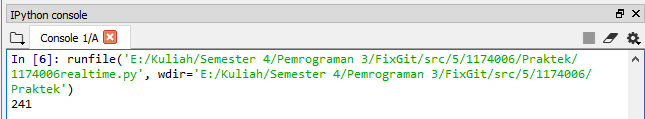
\includegraphics[width=12cm]{figures/5/1174039/Praktek/1.png}
	\centering
	\caption{Hasil dari pembacaan fungsi untuk mendapatkan data dari Arduino.}
\end{figure}

\subsection{Soal No. 2}
Buatlah fungsi (file terpisah/library dengan nama NPMsave.py) untuk mendapatkan data langsung dari arduino dengan looping!
\lstinputlisting[caption = Fungsi untuk mendapatkan data langsung dari Arduino dengan looping., firstline=1, lastline=8]{src/5/1174039/Praktek/1174039save.py}

\begin{figure}[H]
	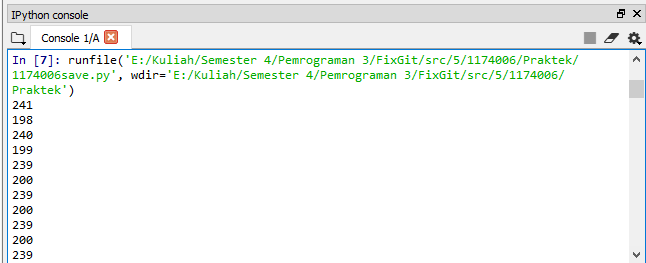
\includegraphics[width=12cm]{figures/5/1174039/Praktek/2.png}
	\centering
	\caption{Hasil dari pembacaan fungsi untuk mendapatkan data dari Arduino dengan looping.}
\end{figure}

\subsection{Soal No. 3}
Buatlah  fungsi  (file  terpisah/library  dengan  nama  NPMrealtime.py) untuk mendapatkan data dari arduino dan langsung ditulis kedalam file csv!
\lstinputlisting[caption = Fungsi untuk mendapatkan data dari Arduino dan langsung ditulis kedalam file CSV., firstline=9, lastline=23]{src/5/1174039/Praktek/1174039realtime.py}

\begin{figure}[H]
	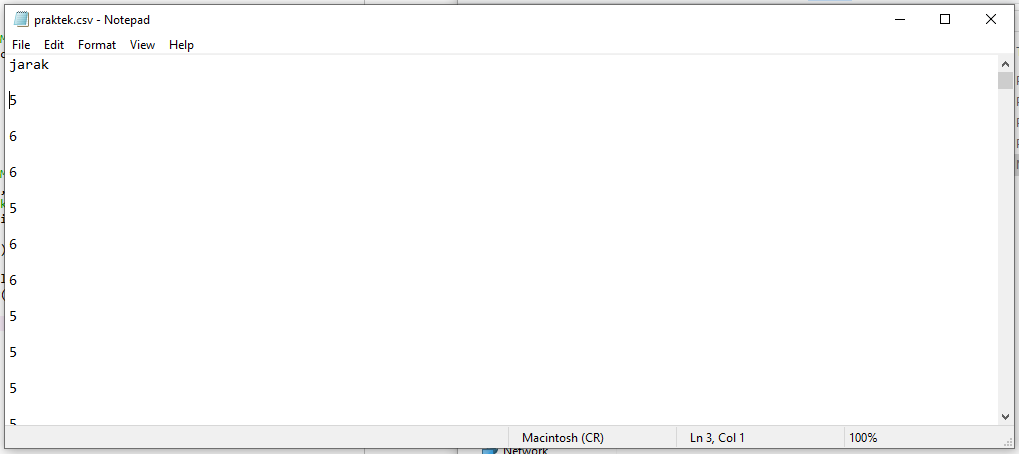
\includegraphics[width=12cm]{figures/5/1174039/Praktek/3.png}
	\centering
	\caption{Hasil dari pembacaan fungsi untuk mendapatkan data dari Arduino dan langsung ditulis kedalam file CSV.}
\end{figure}

\subsection{Soal No. 4}
Buatlah fungsi (file terpisah/library dengan nama NPMcsv.py) untuk membaca file csv hasil arduino dan mengembalikan ke fungsi!
\lstinputlisting[caption = Fungsi untuk membaca file CSV hasil Arduino dan mengembalikan fungsi., firstline=1, lastline=9]{src/5/1174039/Praktek/1174039csv.py}

\begin{figure}[H]
	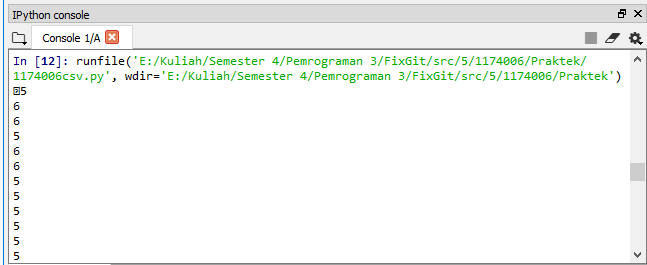
\includegraphics[width=12cm]{figures/5/1174039/Praktek/4.png}
	\centering
	\caption{Hasil dari pembacaan fungsi untuk membaca file csv hasil arduino dan mengembalikan fungsi.}
\end{figure}

\subsection{Kode Program Praktek}
\begin{figure}[H]
	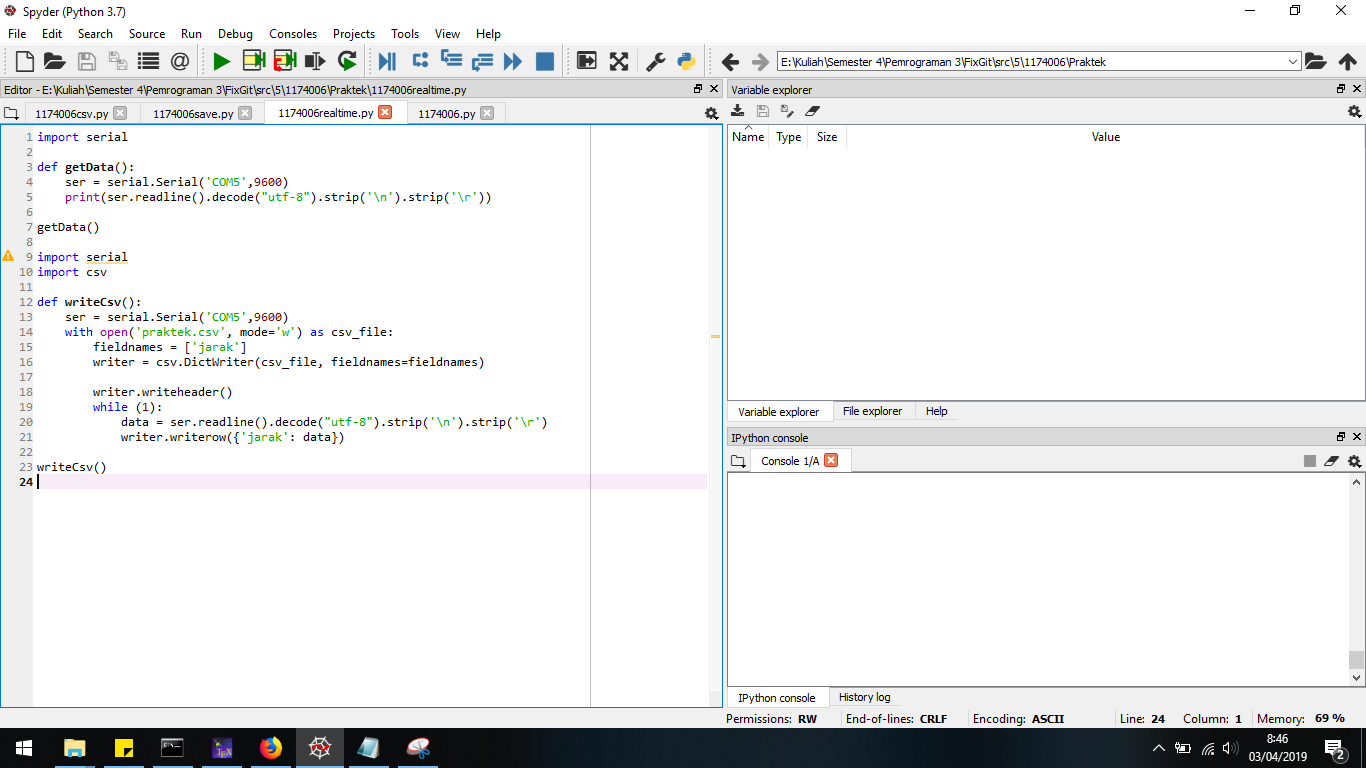
\includegraphics[width=9cm]{figures/5/1174039/Praktek/realtime.png}
	\centering
\end{figure}

\begin{figure}[H]
	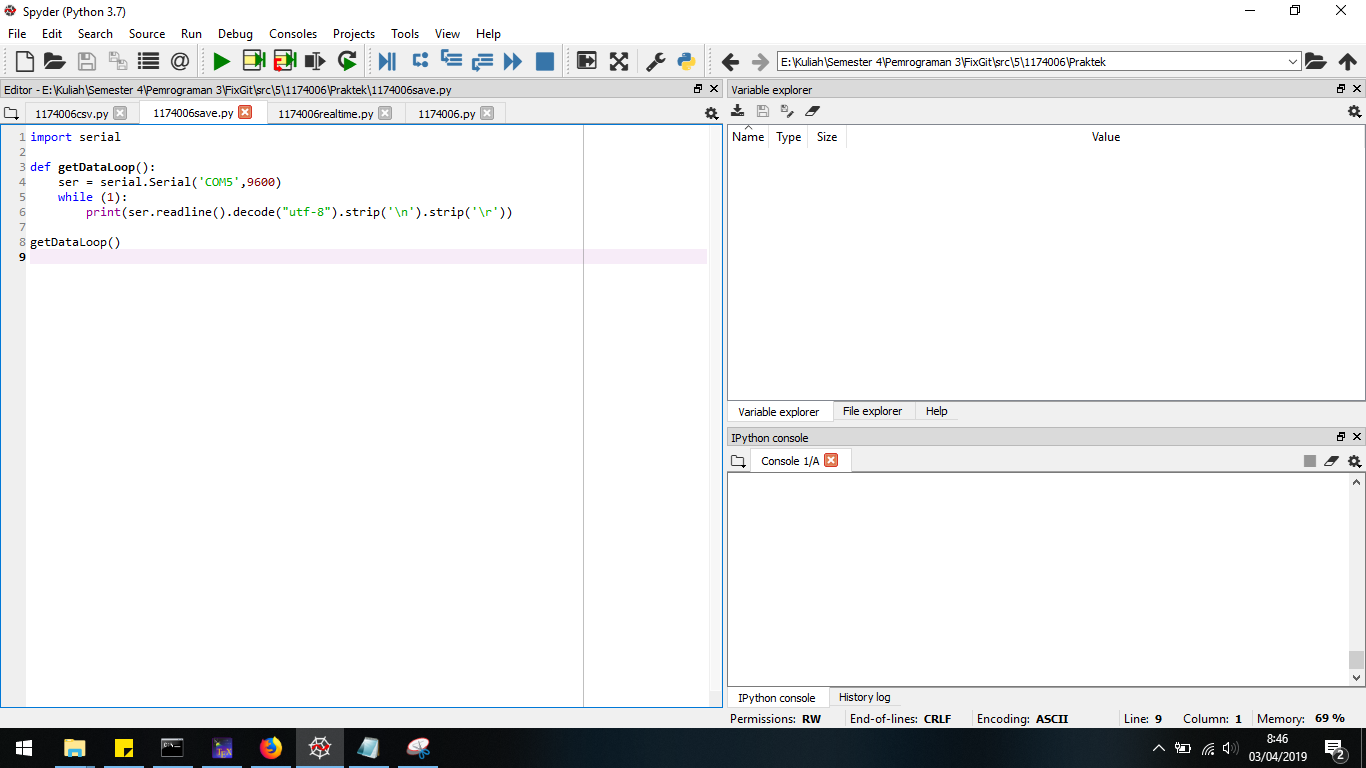
\includegraphics[width=9cm]{figures/5/1174039/Praktek/save.png}
	\centering
\end{figure}

\begin{figure}[H]
	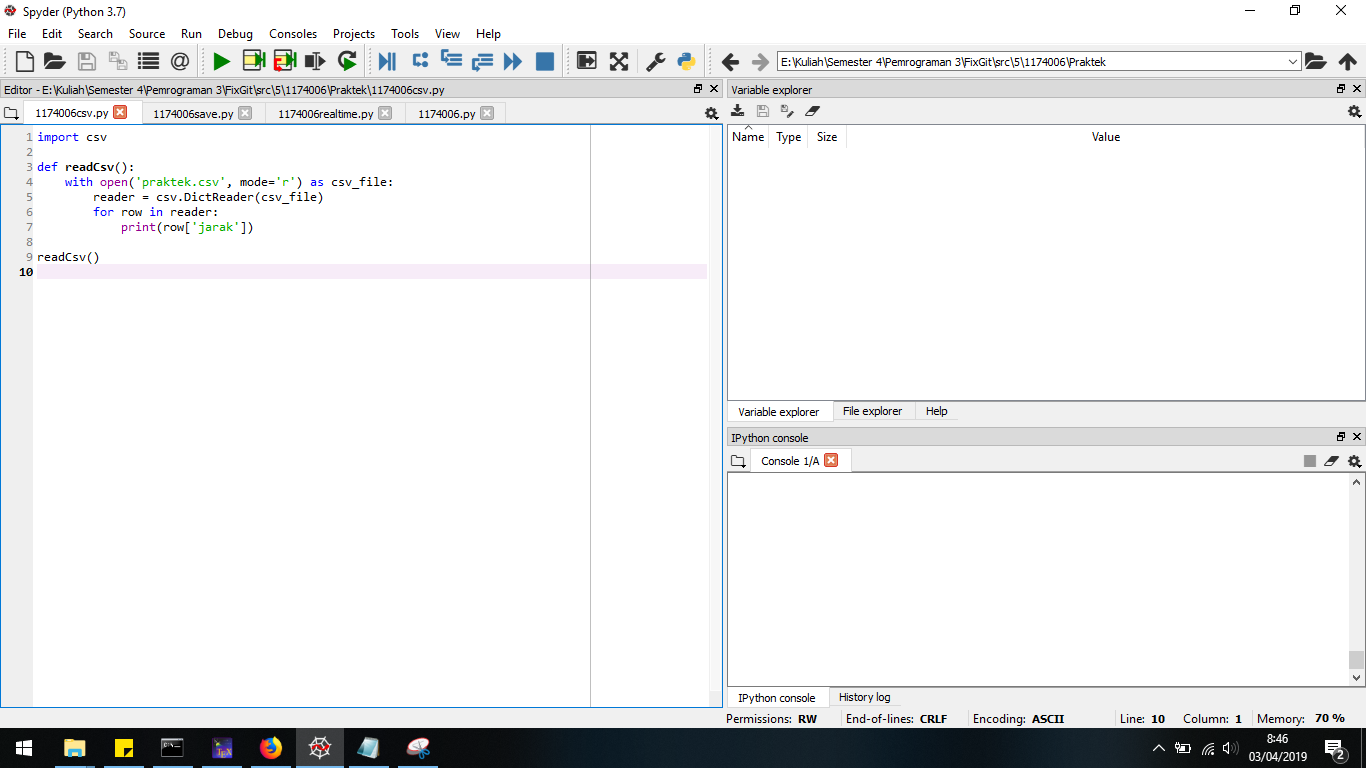
\includegraphics[width=9cm]{figures/5/1174039/Praktek/csv.png}
	\centering
\end{figure}

\subsection{Cek Plagiat Praktek}
\begin{figure}[H]
	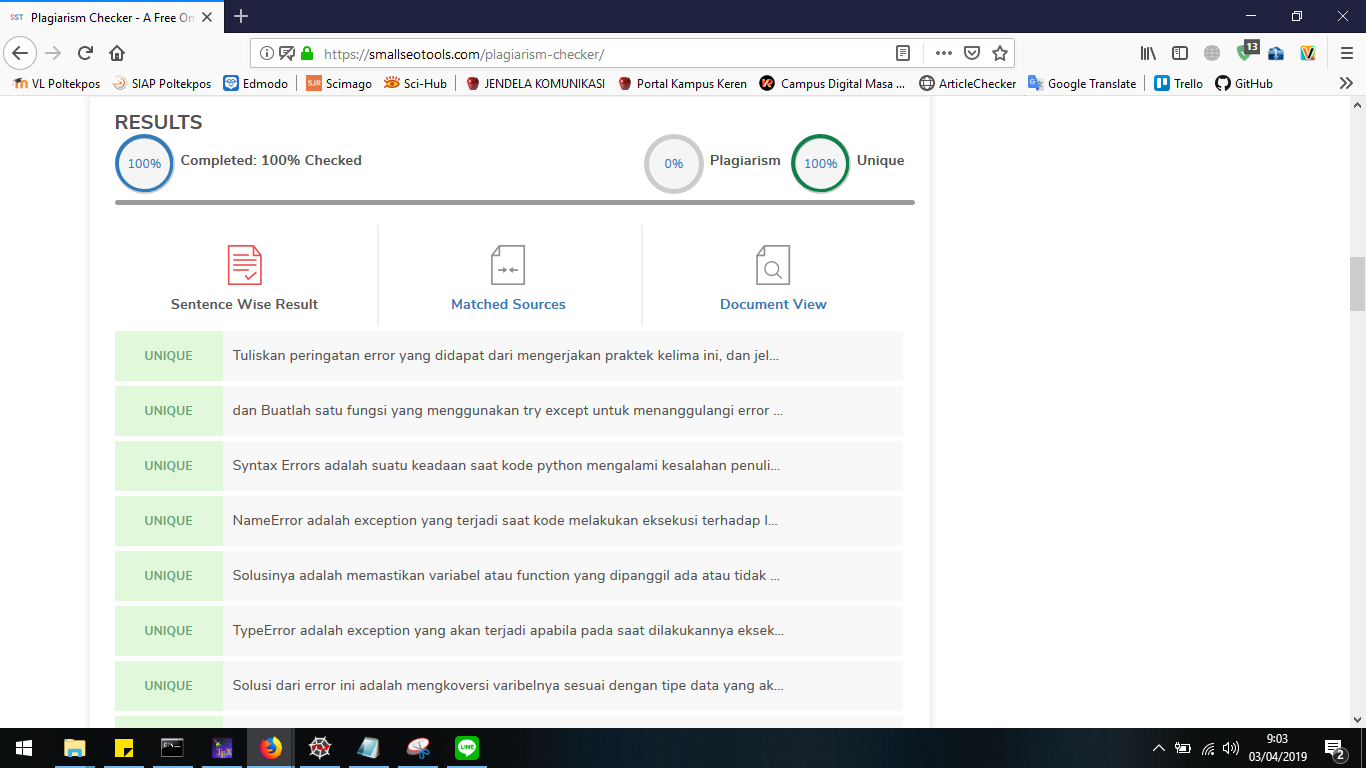
\includegraphics[width=9cm]{figures/5/1174039/Praktek/plagiat.png}
	\centering
\end{figure}

\hfill \break
{\Large \textbf{Ketrampilan Penanganan Error}}

\subsection{Soal No. 1}
Tuliskan  peringatan  error  yang  didapat  dari  mengerjakan  praktek  kelima  ini, dan  jelaskan  cara  penanganan  error  tersebut.   dan  Buatlah  satu  fungsi  yang menggunakan try except untuk menanggulangi error tersebut.

\hfill \break
Peringatan error di praktek kelima ini, yaitu:
\begin{itemize}
	\item Syntax Errors
	Syntax Errors adalah suatu keadaan saat kode python mengalami kesalahan penulisan. Solusinya adalah memperbaiki penulisan kode yang salah.
	
	\item Name Error
	NameError adalah exception yang terjadi saat kode melakukan eksekusi terhadap local name atau global name yang tidak terdefinisi. Solusinya adalah memastikan variabel atau function yang dipanggil ada atau tidak salah ketik.
	
	\item Type Error
	TypeError adalah exception yang akan terjadi apabila pada saat dilakukannya eksekusi terhadap suatu operasi atau fungsi dengan type object yang tidak sesuai. Solusi dari error ini adalah mengkoversi varibelnya sesuai dengan tipe data yang akan digunakan.
\end{itemize}

\hfill \break
Fungsi yang menggunakan try except untuk menanggulangi error.

\lstinputlisting[caption = Fungsi untuk menanggulangi error menggunakan Try Except., firstline=1, lastline=16]{src/5/1174039/Praktek/1174039.py}

\begin{figure}[H]
	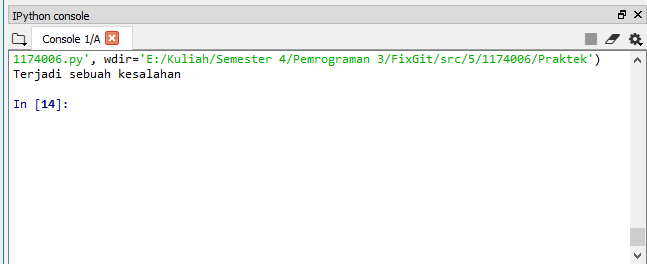
\includegraphics[width=12cm]{figures/5/1174039/Praktek/5.png}
	\centering
	\caption{Hasil pembacaan fungsi untuk menanggulangi error menggunakan Try Except.}
\end{figure}

\subsection{Kode Program Penanganan Error}
\begin{figure}[H]
	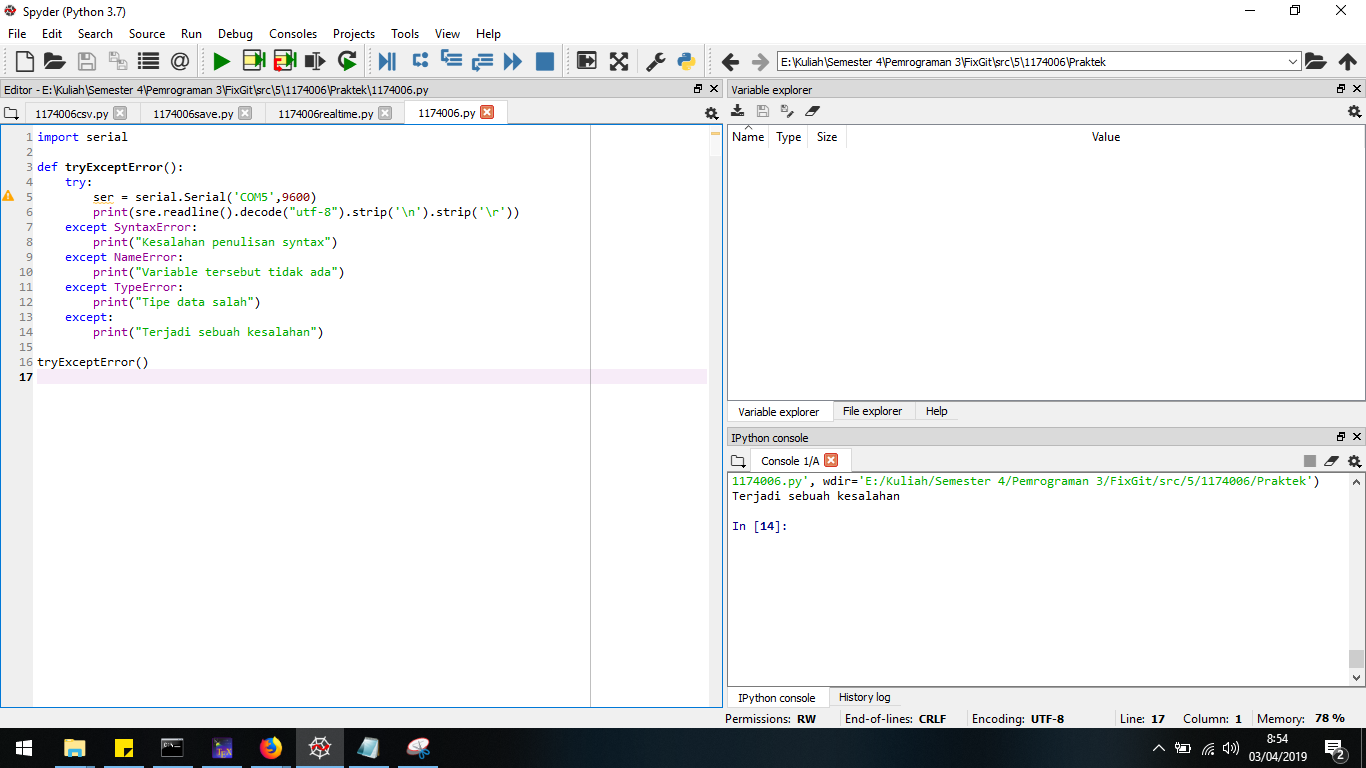
\includegraphics[width=12cm]{figures/5/1174039/Praktek/error.png}
	\centering
\end{figure}

\subsection{Cek Plagiat Penanganan Error}
\begin{figure}[H]
	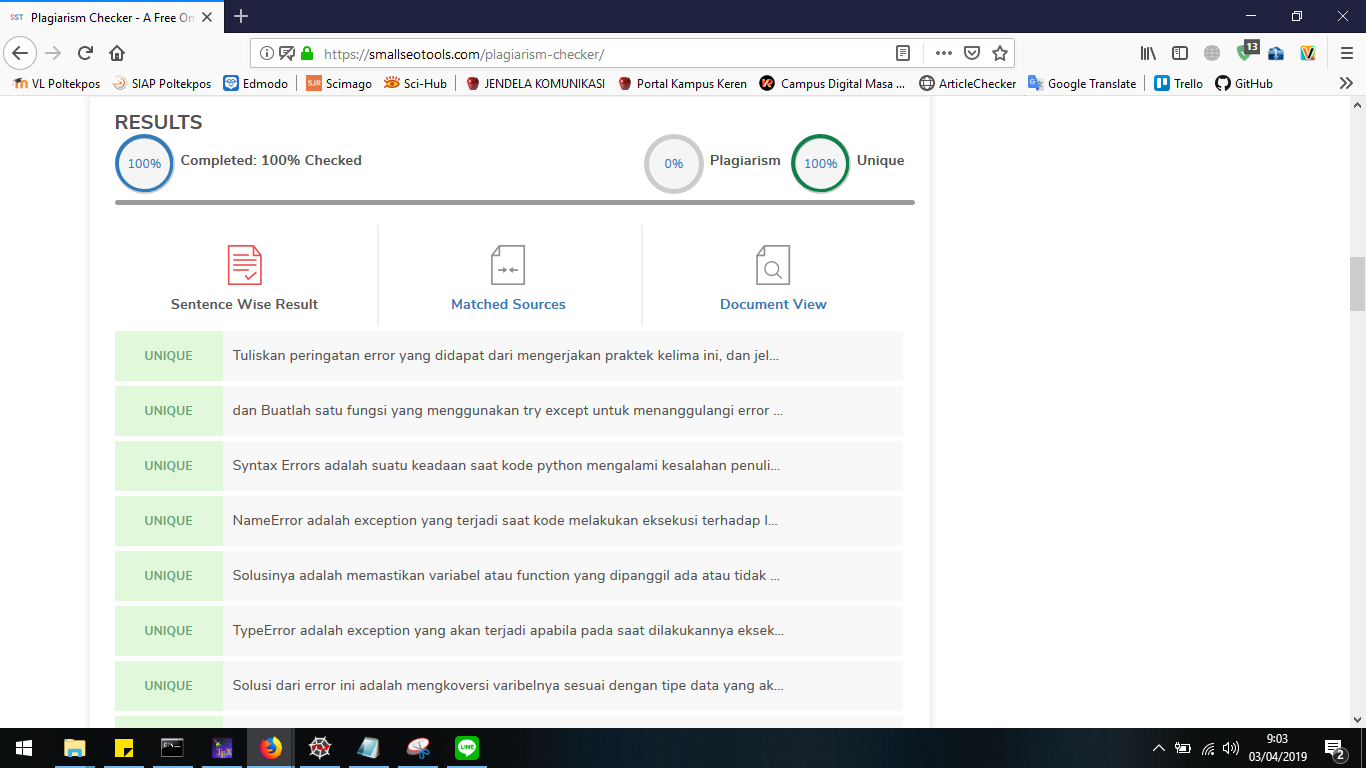
\includegraphics[width=12cm]{figures/5/1174039/Praktek/plagiat.png}
	\centering
\end{figure}